\documentclass{article}

\usepackage{fancyhdr}
\usepackage{extramarks}
\usepackage{amsmath}
\usepackage{amsthm}
\usepackage{amsfonts}
\usepackage{tikz}
\usepackage[plain]{algorithm}
\usepackage{algpseudocode}
\usepackage{enumerate}
\usepackage{tikz}
\usepackage{xifthen}
\usepackage{xparse}
\usepackage{amsmath, amssymb}
\usepackage{lipsum}

\usetikzlibrary{automata,positioning}

%
% Basic Document Settings
%  

\topmargin=-0.45in
\evensidemargin=0in
\oddsidemargin=0in
\textwidth=6.5in
\textheight=9.0in
\headsep=0.25in

\linespread{1.1}

\pagestyle{fancy}
\lhead{\hmwkAuthorName}
\chead{\hmwkClass: \hmwkTitle}
\rhead{\firstxmark}
\lfoot{\lastxmark}
\cfoot{\thepage}

\renewcommand\headrulewidth{0.4pt}
\renewcommand\footrulewidth{0.4pt}

\setlength\parindent{0pt}

%
% Create Problem Sections
%

\newcommand{\enterProblemHeader}[1]{
    \nobreak\extramarks{}{Problem \arabic{#1} continued on next page\ldots}\nobreak{}
    \nobreak\extramarks{Problem \arabic{#1} (continued)}{Problem \arabic{#1} continued on next page\ldots}\nobreak{}
}

\newcommand{\exitProblemHeader}[1]{
    \nobreak\extramarks{Problem \arabic{#1} (continued)}{Problem \arabic{#1} continued on next page\ldots}\nobreak{}
    \stepcounter{#1}
    \nobreak\extramarks{Problem \arabic{#1}}{}\nobreak{}
}

\newcommand*\circled[1]{\tikz[baseline=(char.base)]{
		\node[shape=circle,draw,inner sep=2pt] (char) {#1};}}


\setcounter{secnumdepth}{0}
\newcounter{partCounter}
\newcounter{homeworkProblemCounter}
\setcounter{homeworkProblemCounter}{1}
\nobreak\extramarks{Problem \arabic{homeworkProblemCounter}}{}\nobreak{}

%
% Homework Problem Environment
%
% This environment takes an optional argument. When given, it will adjust the
% problem counter. This is useful for when the problems given for your
% assignment aren't sequential. See the last 3 problems of this template for an
% example.
%

\NewDocumentEnvironment{homeworkProblem}{s m}{
    \IfBooleanT{#1}{\newpage}
    \section{Problem \arabic{homeworkProblemCounter} {\small (#2)}}
    \setcounter{partCounter}{1}
    \enterProblemHeader{homeworkProblemCounter}

}{
    \exitProblemHeader{homeworkProblemCounter}
}

%
% Homework Details
%   - Title
%   - Due date
%   - Class
%   - Instructor
%   - Class number
%   - Name
%   - Student ID

\newcommand{\hmwkTitle}{Homework\ \#9}
\newcommand{\hmwkDueDate}{September 18, 2022}
\newcommand{\hmwkClass}{Probability and Mathematical Statistics}
\newcommand{\hmwkClassInstructor}{Professor Ziyu Shao}

\newcommand{\hmwkClassID}{\circled{0}}

\newcommand{\hmwkAuthorName}{Zhu Zhelin}
\newcommand{\hmwkAuthorID}{2021533077}

%
% Title Page
%

\title{
    \vspace{2in}
    \textmd{\textbf{\hmwkClass:\\  \hmwkTitle}}\\
    \normalsize\vspace{0.1in}\small{Due\ on\ \hmwkDueDate\ at 11:59am}\\
   \vspace{2in}\Huge{\hmwkClassID}\\   
   \vspace{2in}
}

\author{
	Name: \textbf{\hmwkAuthorName} \\
	Student ID: \hmwkAuthorID}
\date{}


\renewcommand{\part}[1]{\textbf{\large Part (\alph{partCounter})}\stepcounter{partCounter}\\}

%
% Various Helper Commands
%

% Useful for algorithms
\newcommand{\alg}[1]{\textsc{\bfseries \footnotesize #1}}
% For derivatives
\newcommand{\deriv}[1]{\frac{\mathrm{d}}{\mathrm{d}x} (#1)}
% For partial derivatives
\newcommand{\pderiv}[2]{\frac{\partial}{\partial #1} (#2)}
% Integral dx
\newcommand{\dx}{\mathrm{d}x}
% Alias for the Solution section header
\newcommand{\solution}{\textbf{\Large Solution}}
% Probability commands: Expectation, Variance, Covariance, Bias
\newcommand{\E}{\mathrm{E}}
\newcommand{\Var}{\mathrm{Var}}
\newcommand{\Cov}{\mathrm{Cov}}
\newcommand{\Bias}{\mathrm{Bias}}

\begin{document}

\maketitle
\pagebreak

% Problem 1
\begin{homeworkProblem}{{\color{blue}mention the source of question}, \textit{e.g.}, BH CH0 \#1}
\begin{enumerate}[(a)]
\item  $P(N=n,X=x,Y=y)$$(0\leq x\leq n,0\leq y\leq n,x+y=n,n\geq 0)=P(X=x,Y=y|N=n)P(N=n)=\binom{n}{x}p^{x}(1-p)^{n-x}\frac{e^{-\lambda}\lambda^{n}}{n!}$ since given N and X we can infer what Y is they are not independent. 
\item $P(N=n,X=x)(0\leq x\leq n,n\geq 0)=P(X=x|N=n)P(N=n)$ which is $\binom{n}{x}p^{x}(1-p)^{n-x}\frac{e^{-\lambda}\lambda^{n}}{n!}$ since given n=10,we can know it is impossible that x=15,so they are not independent
\item $P(X=x,Y=y)(0\leq x,0\leq y)=P(X=x,Y=y|N=x+y)P(N=x+y)=\binom{x+y}{x}p^{x}(1-p)^{y} \frac{e^{-\lambda}\lambda^{x+y}}{(x+y)!}=\frac{e^{-\lambda p}(\lambda p)^{x}\cdot e^{-\lambda (1-p)}(\lambda(1-p))^{y}}{x!\cdot y!}=h(x)\cdot h(y)$so they are indepnedent
\item from c we can get that $P(X=x)=\frac{e^{-\lambda}(\lambda p)^{x}}{x!}$then Corr$(N,X)=\frac{Cov(N,X)}{\sqrt{Var(N)\cdot Var(X)}}=\frac{E(NX)-E(N)E(X)}{\sqrt{Var(N)Var(X)}}$ $E(NX)=\sum\limits_{n=0}^{\infty}\sum\limits_{x=0}^{n} \binom{n}{x}p^{x}(1-p)^{n-x}\frac{e^{-\lambda}\lambda^{n}}{n!}nx=\sum\sum np \binom{n-1}{x-1}p^{x-1}(1-p)^{n-1}\frac{e^{-\lambda}(\lambda)^{n}}{n!}n=(n(n-1)+n)p \frac{e^{-\lambda}(\lambda)^{n}}{n!}=p(\lambda^2+\lambda)$$E(N)=Var(N)=\lambda E(X)=Var(X)=\lambda p$ so the answer is $\sqrt{p}$
\end{enumerate}
	
\end{homeworkProblem}

% Problem 2
\begin{homeworkProblem}*{BH CH0 \#2}
\begin{enumerate}[(a)]
	\item It is Multivariate Normal since $t_1X+t_2 Y+t_3(X+y)=(t_1+t_3)X+(t_2+t_3)Y$  a linear combination of X and Y,so they are Multivariate norma
	\item No If $t_1=t_2=1,t_3=1$then the sum of them is $(1+S)(X+Y)$ $P((1+S)(X+Y)=0)$ It is equal to add the possibility that $S=-1$ and X+Y=0,the total probability is $\frac{1}{2}$ so it isn't Multivariate
	\item First I want to show that if X is $N(0,1)$ then $SX $is also $N(0,1)$,$P(SX=k)=P(X=k|S=1)P(S=1)+P(X=-k|S=-1)P(S=-1)=P(X=k)$(according to the symmetry)so SX is also $N(0,1)$ so SX and SY is also $i.i.d$$N(0,1)$ the linear combination of two $i.i.d N(0,1)$ are also a normal distribution,so it is Multivariate normal 
\end{enumerate}

\end{homeworkProblem}


\begin{homeworkProblem}*{BH CH0 \#3}
	\begin{enumerate}[(a)]
	\item $Corr(X,Y)=\frac{Cov(X,Y)}{\sqrt{Var(X)Var(Y)}}=\rho$ so $Cov(X,Y)=\rho \sigma_1\sigma_2$ if $X$ and $Y-cX$ is independent $Cov(X,Y-cX)=Cov(X,Y)-cCov(X,X)=Cov(X,Y)-cVar(X)=0$,c=$\frac{\rho\sigma_2}{\sigma_1}$
		\item since $T=X+Y,W=X/Y$ $X=\frac{WT}{W+1},Y=\frac{T}{W+1}$
		\begin{equation}
		\begin{vmatrix}
		\frac{\partial X}{\partial T} & \frac{\partial X}{\partial W} \\
		\frac{\partial Y}{\partial T} &\frac{\partial Y}{\partial W}
		\end{vmatrix}=-\frac{T}{(W+1)^2}
	\end{equation}
	so the jocabbian is $\frac{T}{(W+1)^2}$ $f_{T,W}(t,w)=(\lambda)^2 e^{-\lambda t} \frac{t}{(w+1)^2}(0\leq t,0\leq w) $ the marginal pdf $f_T(t)=\int _{0}^{\infty}\lambda^{2}e^{-\lambda t}t \frac{1}{(w+1)^2}dw=\lambda ^{2}e^{-\lambda t}t$,$f_{W}(w)=\frac{1}{(w+1)^2}$
	\item $P(W=w)=P(X=w-t|Y+Z=t)P(Y+Z=t)$ we can know that \begin{equation}	
		P(Y+Z=t)=\begin{cases}
			t(0\leq t \leq 1)\\
			2-t(1\leq t\leq 2)
			0 (other)
		\end{cases}
	\end{equation}
	$(min(w,2)\geq t\geq max(0,w-1))$ 
	then to calculate it \begin{equation}
		\begin{cases}
			\frac{1}{2}w^2 (0\leq w\leq 1)\\
			3w-w^{2}-\frac{3}{2}(1\leq w \leq 2)\\
			\frac{w^2-6w+9}{2}(2\leq w\leq 3)\\
		0(other)	
	\end{cases}
	\end{equation}	
\end{enumerate}
\end{homeworkProblem}
\begin{homeworkProblem}*{BH CH0 \#4}
	\begin{enumerate}[(a)]
\item $P(U_{(j)}=x,U_{(k)}=y)(0\leq x\leq y\leq 1)$ we can use the axis
\begin{figure}[htbp]
	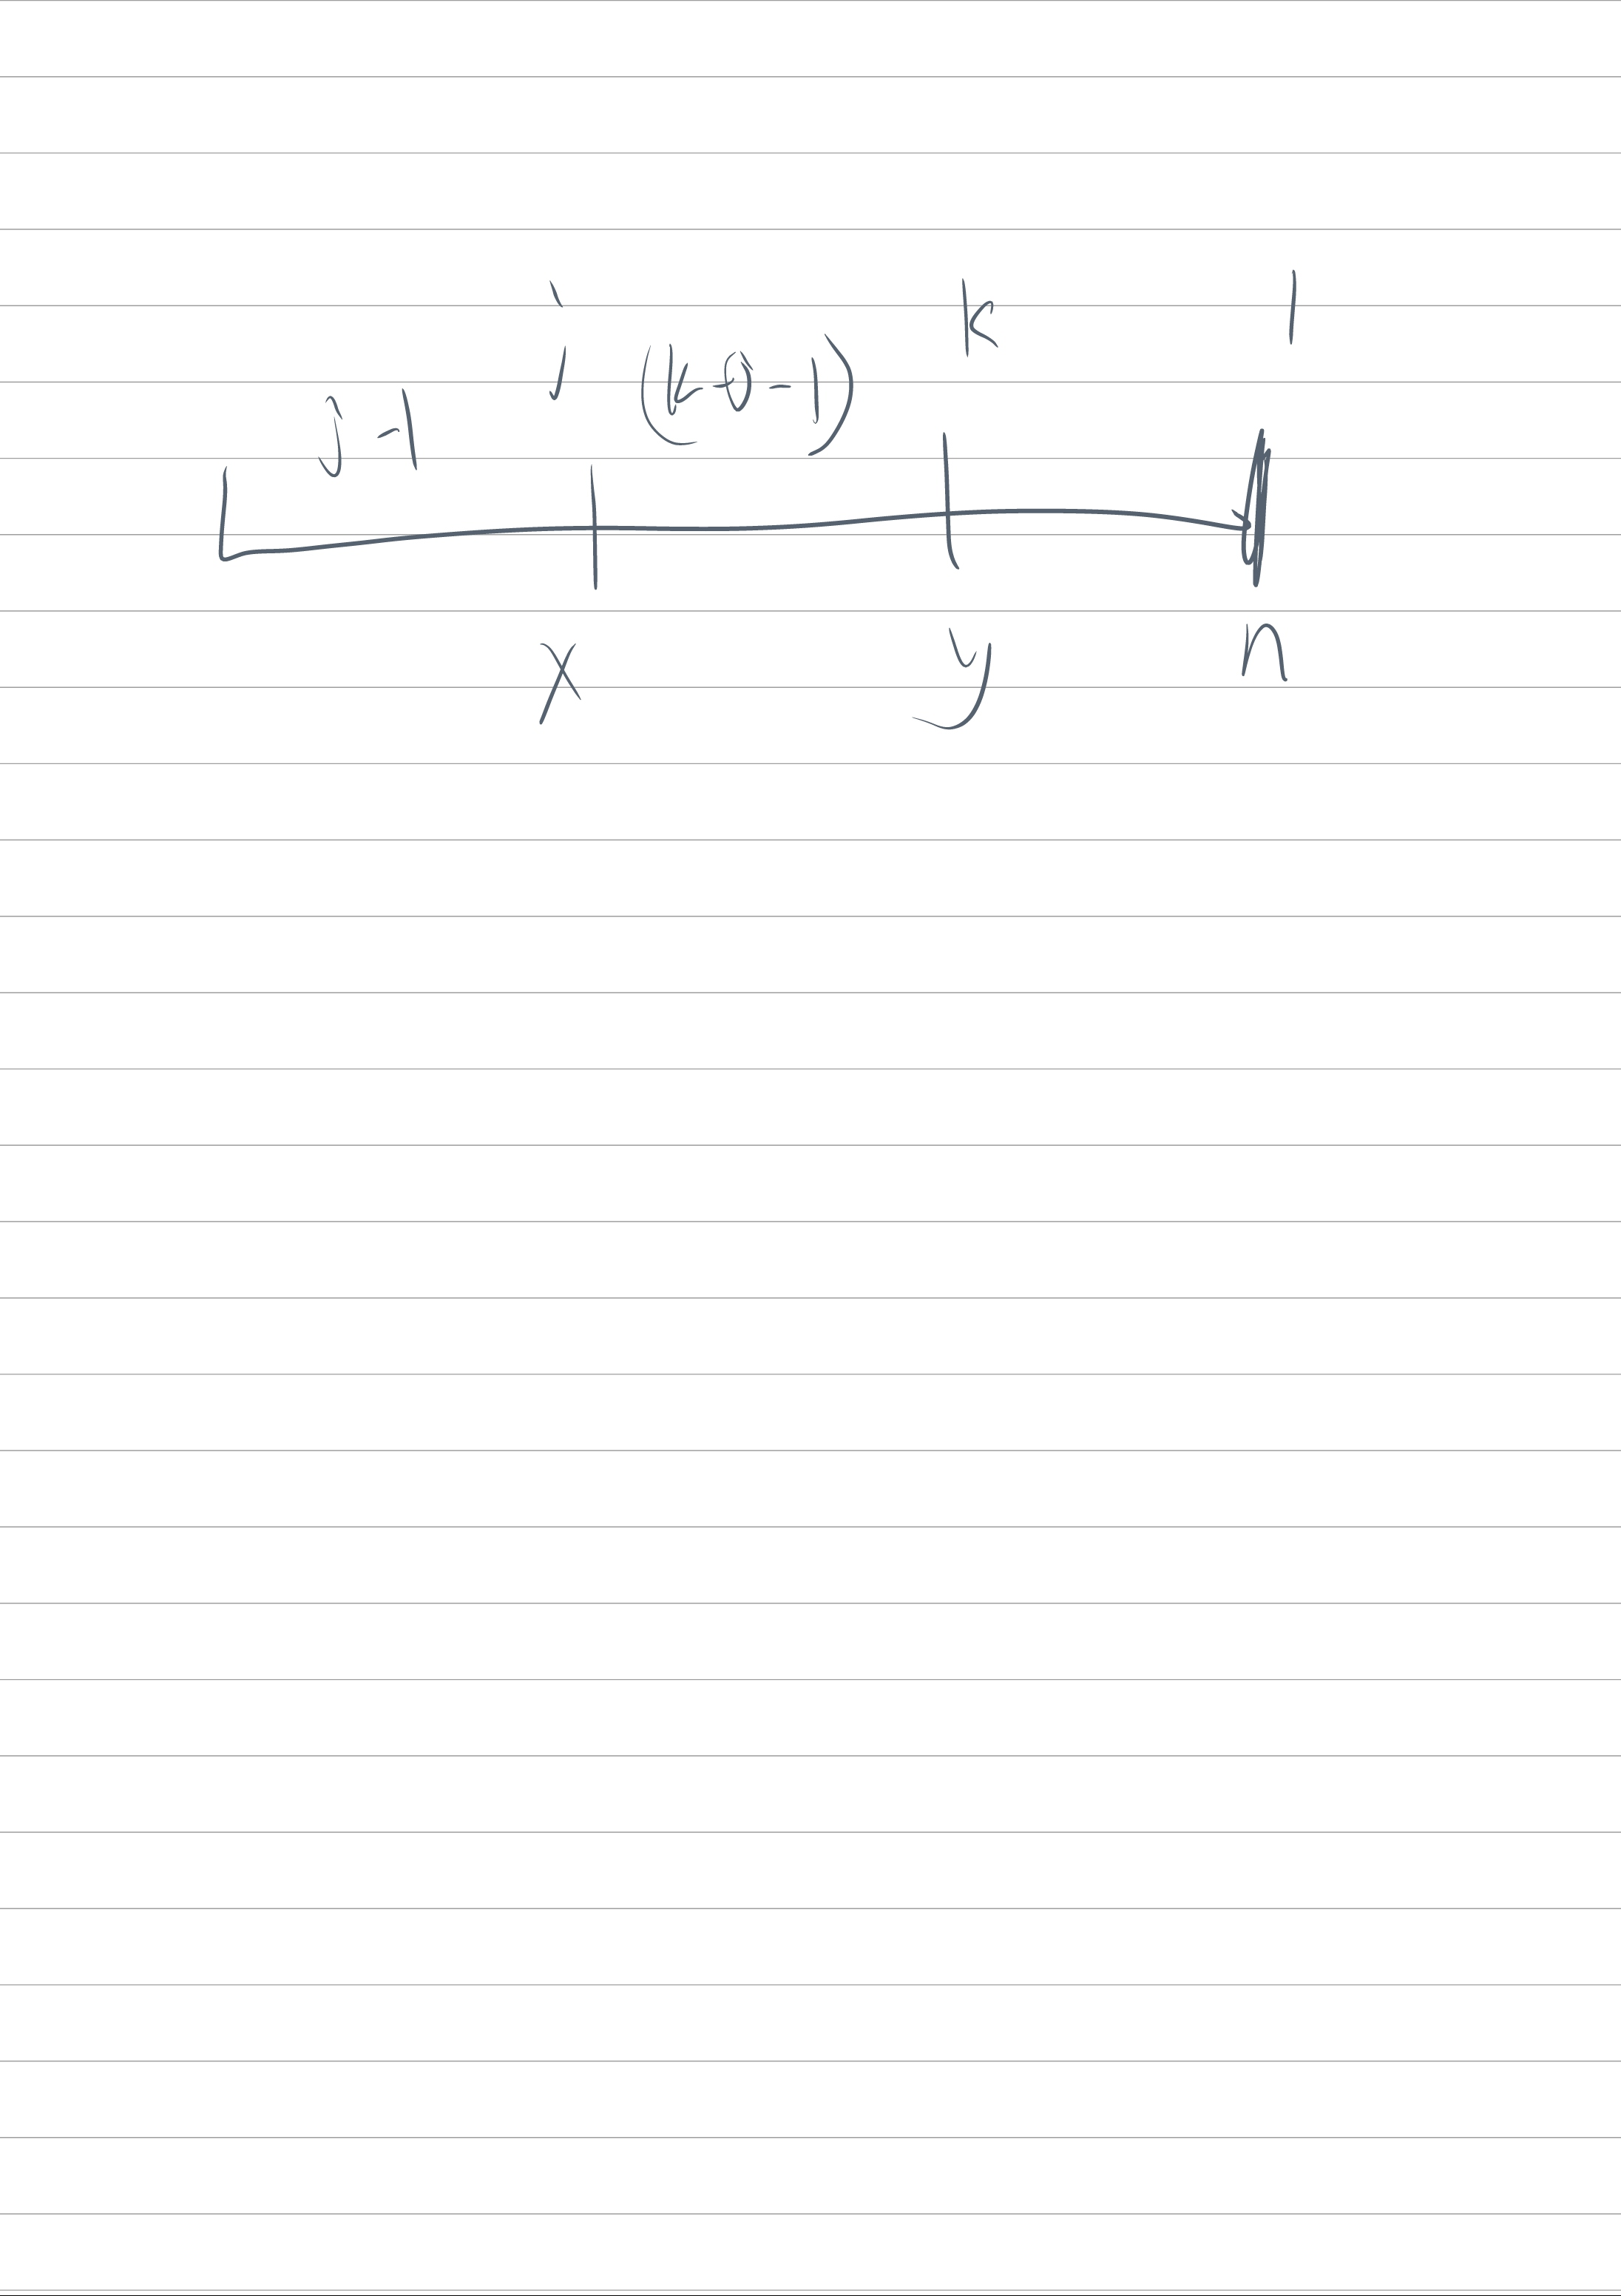
\includegraphics[width=0.5\linewidth,height=0.3\linewidth]{p4.png}
\end{figure}
\\It is equal to $n(n-1)\binom{n-2}{j-1}\binom{n-j-1}{k-j-1}P(X\leq x)^{j-1}P(x\leq X\leq y)^{k-j-1}P(y\leq X\leq 1)^{n-k}=n(n-1)\binom{n-2}{j-1}\binom{n-j-1}{k-j-1}x^{j-1}(y-x)^{k-j-1}(1-y)^{n-k}$
\item considering $U_1,U_2,\cdots,U_n$ are all $i.i.d$ $Unif(0,1)$ we can see $U_i\leq p$ as a success,so the number of success is greater than j is equal to "at least j of the $U_1,U_2\cdots U_n$  $P(U_(j)\leq p)$" $f_{U_{(j)}}(x)=n\binom{n-1}{j-1}x^{j-1}(1-x)^{n-j}=f_{B}(x)$	
then $P(X\geq j)=P(B\leq p)$
\item defining $U_i\leq x$ as success,the lefthandside can be interpreted as all possibility of at least $j$ success happen,from the possition 0 to possition x,the righthandside is the sum of possibility of $P(U_(j)\leq x)$ since at least j success happen is equal to the $j_{th}$ min is smaller than x,so the both side are equal 
\item from c to take the limit you will see the answer,first the rhs $${\lim_{n\to \infty}\sum_{i=j}^{\infty}\binom{n}{i}}x^{k}(1-x)^{n-j}$$ let nx$=\lambda$ since the binom can be approximated as Pois$(\lambda)$ ,and j to be k+1,so during the process the rhs can be wirtten as $Pois(\lambda)$ process ,$P(X\geq k+1)=1-P(X\leq k)$   
then to calculate the lhs since x=$\frac{\lambda}{n}$ let u to be $nt$,j=k+1,the left is $\int_{0}^{\lambda}\frac{n!}{k!(n-k-1)!}(\frac{u}{n})^{k}(1-\frac{u}{n})^{n-k-1}d\frac{u}{n}=\lim_{n\to \infty}\int_{0}^{\lambda}\frac{\Gamma(k+1)n!u^{k}(1-\frac{u}{n})^{n-k-1}}{(n-k-1)!n^{k+1}}du=\int _{0}^{\lambda}\frac{u^{k}e^{-t}}{\Gamma(k+1)}du=1-P(Z\geq \lambda)$
so lhs is equal to rhs
\\using the story we can know that the lhs can be represented as a total length of $\lambda$  let $X_1,X_2,X_3\cdots X_n$ be the iid $Expo(1)$ then think the length of $\lambda$ $P(X\leq k)$ is equal to in the length of $\lambda$,there are at most k arrive,while Gamma$(k+1,1)$,is the total arrival time of $k+1$ iid random variables $P(Z> \lambda)$ means when k+1 arrive the time is larger than $\lambda$ which is the same as at most k arrive happen in the length of $\lambda$   
\end{enumerate}
\end{homeworkProblem}
\begin{homeworkProblem}*{BH CH0 \#5}
	\begin{enumerate}[(a)]
\item 		$E(p^{2}(1-p)^{2})=\int \limits_{0}^{1}\frac{p^{a+1}(1-p)^{b+1}dp}{\beta(a,b)}=\frac{\beta(a+2,b+2)}{\beta(a,b)}=\frac{\Gamma(a+2)\Gamma(b+2)\Gamma(a+b)}{\Gamma(a+b+4)\Gamma(a)\Gamma(b)}=\frac{(a+1)a(b+1)b}{(a+b+3)(a+b+2)(a+b+1)(a+b)}$
\item my posterior distribution for p doen't depend on the specific order of outcomes(due to the consistence of bayes'rule ) if we use the success to update the posterior distribution $\beta(a+1,b)$,if fail update$\beta(a,b+1)$,so that we can the final distribution unrelated to order.
\item from the analysis before we can get p as $\beta(7,5)$since the initial posterior p is $Unif(0,1)$ satisfy $\beta(1,1)$
\item conditional on p ,the first trial and second trial is conditionally  independent as the p is fixed,it is two independent bernouli trials,they are uncorrelated, while conditional on historical data ,the indicator of first success is positively related,since if first success,the p will be larger,which means the second success will more likely to happen.
\item it is same as the possibility of tie happen in the $4_{th}$ they are tie,$\binom{4}{2}p^{2}(1-p)^{2}$ the p is updated by c $\beta(7,5)$ then from a we can know $\binom{4}{2}\frac{8\cdot 7\cdot 6\cdot 5}{12 \cdot 13\cdot 14\cdot 15}=\frac{4}{13}$
\end{enumerate}
\end{homeworkProblem}

\begin{homeworkProblem}*{BH CH0 \#6}

\end{homeworkProblem}

\end{document}
